\section{3 JJ qubit \label{subsec:l33jj}}
\begin{framed}\noindent
  From \cite{gu2017}:
  \begin{itemize}
  \item To  create a double potential  well we need $  \alpha > 0.5 $  and to
    reduce flux noise we need $ \alpha < 0.7 $;
  \end{itemize}

\end{framed}

\begin{figure}[h]
  \centering 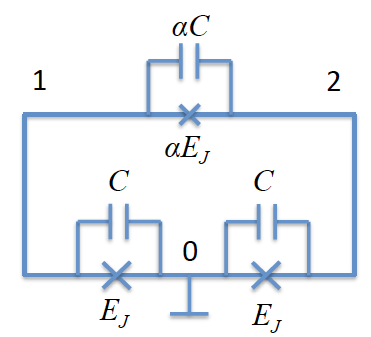
\includegraphics[height=4cm]{3jj}
  \label{fig:l33jj}
\end{figure}

\begin{enumerate}
\item \textbf{\red{Potential energy}} comes from all three JJs, where we
  denote the phases

  \begin{equation}
    e^{i\phi_{01}} = e^{i(\phi_0-\phi_1)}
  \end{equation}

  \blue{\begin{equation}
      \begin{aligned}
        U_{\text{potential}} & = E_J(1-\cos(\phi_{01})) + \alpha E_J(1-\cos(\phi_{12})) + E_J(1-\cos(\phi_{20}))\\
        &  = E_J\bigg[2+\alpha  -  \cos(\phi_{01})  - \cos(\phi_{20})  -
        \alpha\cos(\phi_\text{ext}-\phi_{01} - \phi_{20})\bigg].
      \end{aligned}
    \end{equation}}

  \begin{figure}[ht]
    \centering 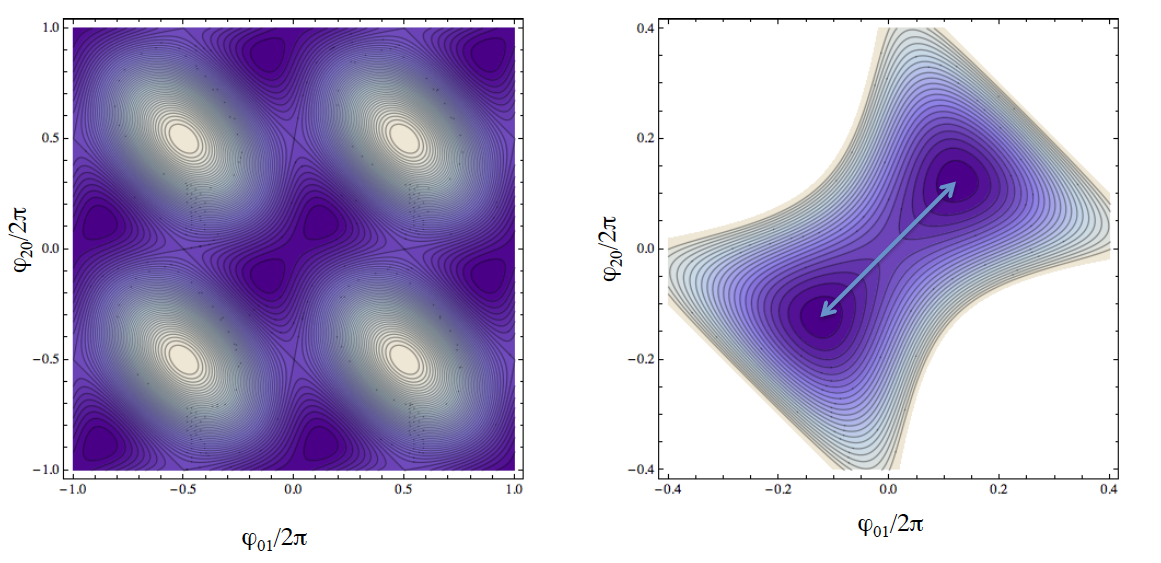
\includegraphics[height=4cm]{3jjc}%
    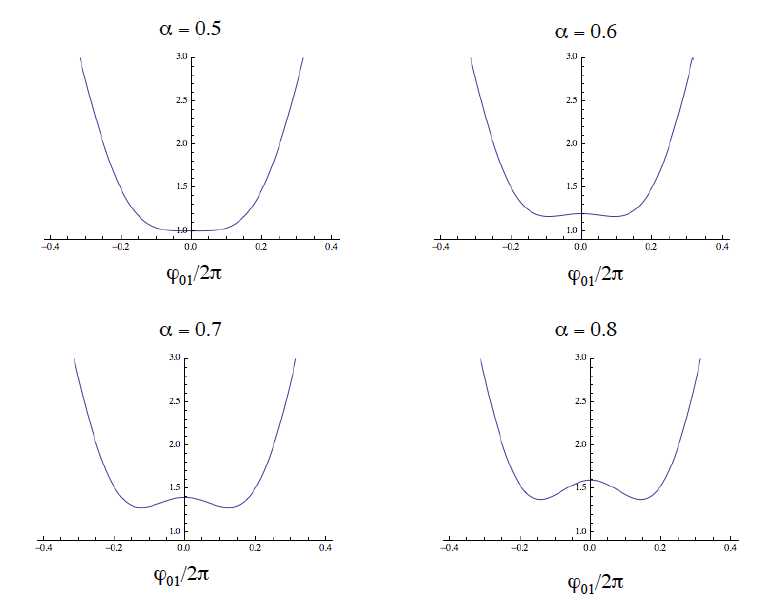
\includegraphics[height=5cm]{3jj1}%
    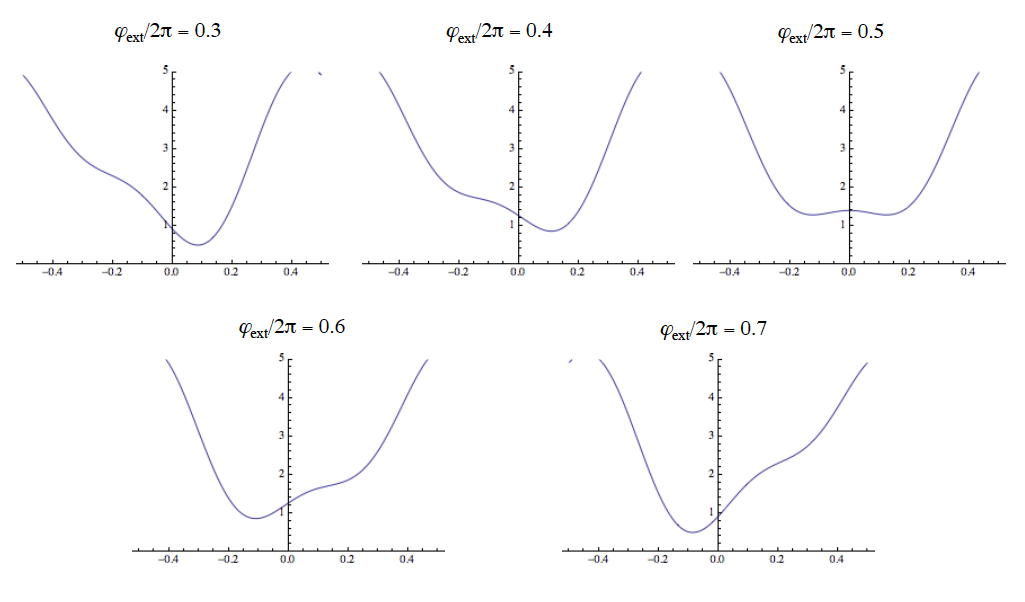
\includegraphics[height=5cm]{3jj2}%
    \caption{$\alpha$ determines the height of the barrier in the middle
      of  the   two  wells.   Larger   alpha  raises  the   barrier  up.
      $ \phi_\text{ext}  $ determines the  symmetry of the wells  (as in
      the previous section).}
  \end{figure}

\item  \red{\textbf{The   kinetic  energy}}  comes  from   the  charging
  energy. Its better to work with  the capacitance matrix for the system
  which links a given charge vector  $ \vec{n} $ with a potential vector
  $ \vec{V} $

  \begin{equation}
    \left\lbrace \begin{aligned}
        \vec{n} & = \left(\begin{smallmatrix}
            n_1\\n_2
          \end{smallmatrix}\right)\\
        \vec{V} & =\left(\begin{smallmatrix} V_1\\V_2
          \end{smallmatrix}\right)\\
        C & = \left(\begin{smallmatrix} C_{01}+C_{12} & -C_{12}\\-C_{12}
            &C_{02}+C_{12}
          \end{smallmatrix}\right)\\
      \end{aligned}\right.  \Rightarrow \vec{n} = \frac{C\vec{V}}{2e}
    \equiv \begin{bmatrix}
      C_{01}\left(V_1-0\right)   +  C_{12}\left(V_1-V_2\right)\\   C_{01}\left(V_2-0\right)  +
      C_{12}\left(V_2-V_1\right)
    \end{bmatrix},
  \end{equation}

  \noindent  which  is  just  the  typical evaluating  of  charge  on  a
  capacitor from $ Q = CV $.  For evaluating the kinetic energy from the
  charges

  \begin{equation}
    \left\lbrace \begin{aligned}
        \vec{V} & = 2eC^{-1}\vec{n}\\
        \vec{Q} & = 2e\vec{n}\\
        \red{U_{\text{kinetic}}} & \red{= \frac{1}{2}Q.V}\\
      \end{aligned}\right.  \Rightarrow \red{U_{\text{kinetic}} =
      \frac{1}{2}\left(2e\vec{n}^{\text{T}}\right)\left(2eC^{-1}\vec{n}\right)               =
      \frac{(2e)^2}{2}\vec{n}^{\text{T}}C^{-1}\vec{n}},
  \end{equation}


\item The total Hamiltonian for the 3JJ/3 capacitor system being

  \begin{equation}
    \label{eqn:l23JJ}
    \begin{aligned}
      \mathcal{H}       &       =       \red{U_{\text{kinetic}}}       +
      \blue{U_{\text{potential}}}\\                  &                 =
      \red{\frac{(2e)^2}{2}\vec{n}^{\text{T}}C^{-1}\vec{n}}            +
      \blue{E_J\bigg[2+\alpha  -  \cos(\phi_{01})  -  \cos(\phi_{20})  -
        \alpha\cos(\phi_\text{ext}-\phi_{01} - \phi_{20})\bigg]}.
    \end{aligned}
  \end{equation}

  For  simple representation  in matrix  form, we  write it  out in  the
  \textbf{charge    basis}.    In    such   a    basis   (recall    from
  Eq.\eqref{eqn:l2-phase} for the  one island case) we  have the results
  summarised in Table \ref{tab:phaseChange}.

  {\begin{table}[h]
      \label{tab:phaseChange}
      \caption{Note how  the phase  operators increase and  decrease the
        islands associated to a given phase.}
      \begin{center}
        {\footnotesize \begin{tabular}{|c|c|} \hline \textbf{One island}
            (Sec.\ref{subsec:l2-CPB})     &      Two     islands\\\hline
            $      \hat{N}      =     \sum_N\iketbra{N}{N}      $      &
            $ \frac{(2e)^2}{2}\begin{pmatrix} n_1 & n_2
            \end{pmatrix}C^{-1}\begin{pmatrix}n_1 \\  n_2\end{pmatrix} =
            \displaystyle\sum_{N_1,N_2}\mathbf{U}(n_1,n_2)\iketbra{n_1,n_2}{n_1,n_2}
            $\\\hline
                         \multirow{3}{*}{$ e^{i\phi}  = \sum_N\iketbra{N+1}{N}$} & $ e^{i\phi_{01}} = e^{i(\phi_{0}-\phi_1)} =  \displaystyle\bigg[\sum_{n_1}\iketbra{n_1-1}{n_1}\bigg]\otimes \red{\bigg[\sum_{n_\text{ground}}\iketbra{n_\text{ground}+1}{n_\text{ground}}\bigg] - \text{ ignore}}$\\
                                          & $ e^{-i\phi_{01}} = e^{i(\phi_{1}-\phi_0)} =  \displaystyle\sum_{n_1}\iketbra{n_1+1}{n_1}$\\
                                          & $ e^{i\phi_{20}} = e^{i(\phi_{2}-\phi_0)} =  \displaystyle\sum_{n_2}\iketbra{n_2+1}{n_2}$\\
                         \multirow{3}{*}{$ e^{-i\phi}  = \sum_N\iketbra{N-1}{N}$} & $ e^{-i\phi_{20}} = e^{i(\phi_{0}-\phi_2)} =  \displaystyle\sum_{n_2}\iketbra{n_2-1}{n_2}$\\
                                          & $ e^{i\phi_{12}} (\equiv e^{\phi_\text{ext}-\phi_{01}-\phi_{20}}) = e^{i(\phi_1-\phi_2)} =  \displaystyle\bigg[\sum_{n_1}\iketbra{n_1+1}{n_1}\bigg]\otimes {\bigg[\sum_{n_2}\iketbra{n_2-1}{n_2}\bigg]} $\\
                                          &
                                            $      e^{-i\phi_{12}}     =
                                            e^{i(\phi_2-\phi_1)}       =
                                            \displaystyle\bigg[\sum_{n_1}\iketbra{n_1-1}{n_1}\bigg]\otimes
                                            {\bigg[\sum_{n_2}\iketbra{n_2+1}{n_2}\bigg]}
                                            $\\\hline
                       \end{tabular}}
                   \end{center}
                 \end{table}}

             \item We draw  parallels to rewrite our  new Hamiltonian in
               matrix  form  (using  exponential form  of  trigonometric
               functions and zeroing constant  offsets and replacing the
               last exponential  with explicit  dependence on  the phase
               across the junction)

               \begin{equation}
                 \label{eqn:l3ToMatrixForm}
                 \begin{aligned}
                   \mathcal{H}  = \red{\frac{(2e)^2}{2}\vec{n}^{\text{T}}C^{-1}\vec{n}} & - \blue{\frac{E_J}{2}\big(e^{i\phi_{01}}+e^{-i\phi_{01}}\big) - \frac{E_J}{2}\big(e^{i\phi_{20}}+e^{-i\phi_{20}}\big) - \frac{\alpha E_J}{2}\big(e^{i\phi_{12}}+e^{-i\phi_{12}}\big)}\\\\
                   \Rightarrow \sum_{n_1,n_2} \red{U(n_1,n_2)\iketbra{n_1,n_2}{n_1,n_2}} & \\
                   & \blue{ - \frac{E_J}{2}\bigg[\iketbra{n_1-1}{n_1}+\iketbra{n_1+1}{n_1}\bigg]\otimes \mathbb{I}_2}\\
                   & \green{- \frac{E_J}{2} \mathbb{I}_1\otimes\bigg[\iketbra{n_2+1}{n_2}+\iketbra{n_2-1}{n_2}\bigg]}\\
                   & \purple{- \frac{\alpha E_J}{2}\bigg[\iketbra{n_1+1}{n_1}\iketbra{n_2-1}{n_2}+\iketbra{n_1-1}{n_1}\iketbra{n_2+1}{n_2}\bigg]}\\
                   \Rightarrow \sum_{n_1,n_2} \red{U(n_1,n_2)\iketbra{n_1,n_2}{n_1,n_2}} & \\
                   & \blue{ - \frac{E_J}{2}\bigg[\iketbra{n_1-1,\mathbf{n_2}}{n_1,\mathbf{n_2}}+\iketbra{n_1+1,\mathbf{n_2}}{n_1,\mathbf{n_2}}\bigg]\ira \text{ $n_2$ constant}}\\
                   & \green{- \frac{E_J}{2} \bigg[\iketbra{\mathbf{n_1},n_2+1}{\mathbf{n_1},n_2}+\iketbra{\mathbf{n_1},n_2-1}{\mathbf{n_1},n_2}\bigg]\ira \text{ $n_1$ constant}}\\
                   &                \purple{-               \frac{\alpha
                       E_J}{2}\bigg[\iketbra{n_1+1,n_2-1}{n_1,n_2}+\iketbra{n_1-1,n_2+1}{n_1,n_2}\bigg]}
                 \end{aligned}
               \end{equation}

               \noindent and writing out in matrix form

  \begin{equation}
    \mathcal{H} = \kbordermatrix{
      & \ket{-1,0} & \ket{0,-1} & \ket{0,0} & \ket{0,1} & \ket{1,0}\\
      \bra{-1,0} &\red{ U(-1,0)} & \purple{-\frac{E_J}{2}} & \blue{-\frac{E_J}{2}} & 0 & 0\\
      \bra{0,-1} & \purple{-\frac{E_J}{2}} & \red{U(0,-1) } & \green{-\frac{E_J}{2}} & 0 & 0\\
      \bra{0,0} & \blue{-\frac{E_J}{2}} & \green{-\frac{E_J}{2}} & \red{U(0,0)} & \green{-\frac{E_J}{2}} & \blue{-\frac{E_J}{2}}\\
      \bra{0,1} & 0 & 0 & \green{-\frac{E_J}{2}} & \red{U(0,1) }& \purple{-\frac{E_J}{2}}\\
      \bra{1,0} & 0 & 0 & \blue{-\frac{E_J}{2}} & \purple{-\frac{E_J}{2}} & \red{U(1,0)}\\
    }
  \end{equation}
\end{enumerate}

  \begin{center}
    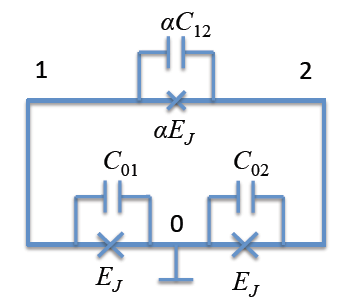
\includegraphics[height=6cm]{3jja}  System  of tunnelling  electrons
    between the three junctions
  \end{center}



  \newpage
